\chapter*{Funciones Lineales y cuadráticas}
\setcounter{chapter}{2}
\setcounter{section}{0}

\section{Concepto de función}
\blueBox{Definición de Función}{
    Se llama \emph{función f} de \emph{A en B} a toda relación que asocia a cada elemento de A un único elemento de B.\\
    El conjunto A se llama \emph{dominio} de f y el conjunto B se llama \emph{codominio} de f.

    $$f: A \rightarrow B$$
}

\section{Función Lineal}
\blueBox{Definición (Función Lineal)}{
    Una función $f: \R \rightarrow \R$ se llama \emph{lineal} si es de la forma
    $$f(x) = ax + b$$
    con $a \in \R$ y $b \in \R$.
}

\paragraph{Gráficas de las funciones lineales}
\begin{itemize}
    \item[1.]Si la pendiente, \emph{a}, es igual a 0, la gráfica es una recta horizontal.
    $$f(x) = b$$
    \begin{center}
        \begin{tikzpicture}
            \begin{axis}[
                axis x line = center,
                axis y line = center,
                xlabel = $x$, ylabel = {$y$}]
                \addplot [ 
                    domain=-10:10, samples=30, color=blue 
                ] {5};
                \node[above right, blue] at (axis cs:0,5) {$f(x) = 5$};
            \end{axis}
        \end{tikzpicture}
    \end{center}
    \item[2.]Si $a \neq 0$, la recta corta al eje vertical (\textbf{eje de cortdenadas}) en el punto (0;$b$), de aquí que el coeficiente $b$ se conoce como \emph{ordenada al origen}.
\end{itemize}

\subsection{Ecuación de la recta que pasa por dos puntos}
Se puede determinar una recta solo sabiendo dos puntos que pertenezcan a ella. Para esto se utiliza la \emph{ecuación general de la recta}:
$$y = mx + b$$


\subsubsection{Ejemplo:} Determinar la ecuación de la recta que pasa por los puntos $P(-1;3)$ y $Q(5;-3)$.
\begin{center}
    \begin{tikzpicture}
        \begin{axis}[
            ymin=-4,
            ymax=4,
            xtick={-1,0,1,3,5},
            ytick={-3,-1,0,1,3},
            axis x line = center,
            axis y line = center,
            xlabel = $x$, ylabel = {$y$}]
            \addplot [ 
                draw=none
            ] coordinates {(0,0) (-2,3) (6,-3)};
            % draw circle at (-1;3)
            \draw[fill=black] (axis cs:-1,3) circle (3pt) node[above right] {$P$};
            \draw[fill=black] (axis cs:5,-3) circle (3pt) node [right] {$Q$};
            \draw[dashed] (0,-3) -- (5,-3) -- (5,0);
            \draw[dashed] (-1,0) -- (-1,3) -- (0,3);
        \end{axis}
    \end{tikzpicture}
    \hspace{1cm}
    \begin{tikzpicture}
    \begin{axis}[
        ymin=-4,
        ymax=4,
        xmin=-2,
        xmax=6,
        xtick={-1,0,1,3,5},
        ytick={-3,-1,0,1,3},
        axis x line = center,
        axis y line = center,
        xlabel = $x$, ylabel = {$y$}]
        \addplot [ 
            color=blue 
        ] {-x+2};
        % draw circle at (-1;3)
        \draw[fill=black] (axis cs:-1,3) circle (3pt) node[above right] {$P$};
        \draw[fill=black] (axis cs:5,-3) circle (3pt) node [right] {$Q$};
        \draw[dashed] (0,-3) -- (5,-3) -- (5,0);
        \draw[dashed] (-1,0) -- (-1,3) -- (0,3);
    \end{axis}
\end{tikzpicture}
\end{center}

\subsubsection{Solución:}
Pasa por $P \rightarrow f(-1) = 3$ y $Q \rightarrow f(5) = -3$.
$$
\begin{cases}
    \phantom{-}3 & = (-1) \cdot a + b \\
              -3 & = 5a + b
\end{cases} 
$$
$$3 \: + \: a = -3 -5a$$
$$6a = -6 \Leftrightarrow a = -1$$
y $b = 2$:
$$f(x) = -x + 2$$

\subsection{Ecuación de la recta conociendo un punto y su pendiente}

Si una recta pasa por el punto $(1;3)$ y su pendiente es -2, conocemos la ecuación de la recta:
$$f(x) = -2x+b$$
Calculamos la ordenada al origen, reemplazando $f(x)$ por 3 y $x$ por 1:
$$3 = -2 \cdot 1 + b \Leftrightarrow 5 = b$$
$$f(x) = -2x + 5$$

\blueBox{Rectas paralelas y perpendiculares}{
    Dadas dos funciones lineales $y = a_1 x + b_1$ e $y = a_2 x + b_2$ sus gráficas son:
    \begin{enumerate}
        \item Paralelas si $a_1 = a_2$
        \item Perpendiculares si $a_1 \cdot a_2 = -1$
    \end{enumerate}
}

\section{Función Cuadrática}

\blueBox{Definición (Función Cuadrática)}{
    Una función $f: \R \rightarrow \R$ se llama \emph{cuadrática} si es de la forma
    $$f(x) = ax^2 + bx + c$$
    con $a, b, c \in \R$ y $a \neq 0$.
}

\begin{center}
\begin{tabular}[b]{c|c}
    $x$ & $f(x) = x^2$ \\
    \hline
    -4 & 16 \\
    -3 & 9 \\
    -2 & 4 \\
    -1 & 1 \\
    \phantom{-}0 & 0 \\
    \phantom{-}1 & 1 \\
    \phantom{-}2 & 4 \\
    \phantom{-}3 & 9 \\
    \phantom{-}4 & 16 \\
\end{tabular}
\hspace{1cm}
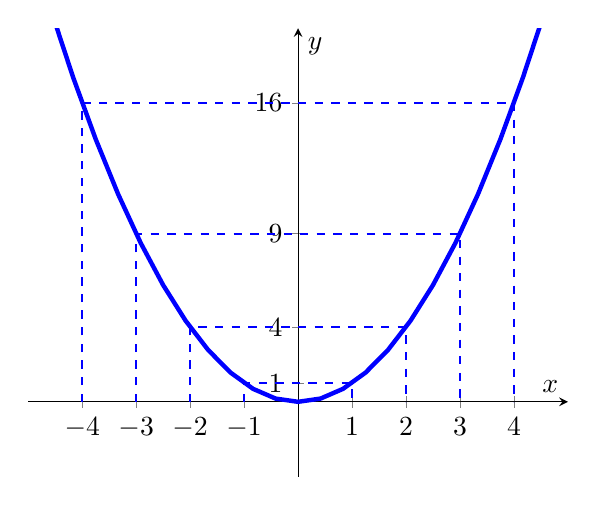
\begin{tikzpicture}
    \begin{axis}[
        ymin=-4,
        ymax=20,
        xmin=-5,
        xmax=5,
        xtick={-4,-3,-2,-1,0,1,2,3,4},
        ytick={0,1,4,9,16},
        axis x line = center,
        axis y line = center,
        xlabel = $x$, ylabel = {$y$}]
        \addplot [ 
            color=blue, ultra thick
        ] {x^2};
        \draw[dashed, thick, blue] (-4,0) -- (-4,16) -- (4,16) -- (4,0);
        \draw[dashed, thick, blue] (-3,0) -- (-3,9) -- (3,9) -- (3,0);
        \draw[dashed, thick, blue] (-2,0) -- (-2,4) -- (2,4) -- (2,0);
        \draw[dashed, thick, blue] (-1,0) -- (-1,1) -- (1,1) -- (1,0);
    \end{axis}
\end{tikzpicture}
\end{center}

Podemos ver que:
\begin{itemize}
    \item El gráfico es simétrico respecto al eje \emph{y}. La recta \emph{x = 0} es el \textbf{Eje se simetría}.
    \item El menor valor que toma la función es 0 y se produce en \emph{x = 0}. Este punto es el \textbf{vértice} de la parábola.
    \item La función es creciente en el intervalo $(-\infty;0)$ y decreciente en el intervalo $(0;\infty)$.
    \item El conjunto imagen de la función es el intervalo $[0;\infty)$ o $\R^+_0$.
\end{itemize}

\subsection{Forma canónica}
Toda función cuadrática, desde su forma polínomica $f(x) = ax^2 + bx +c$, se puede escribir en la forma canónica:
$$f(x) = a(x-h)^2 + k$$
donde $h$ y $k$ son las coordenadas del vértice de la parábola.

\subsubsection{Ejemplo:}
Determinar la ecuación de la función que pasa por el punto (3;-1) y tiene como vértice el punto (-1;4).

\subsubsection{Solución:}
Reemplazamos en la forma canónica:
$$f(x) = a(x+1)^2 + 4$$
Para obtener $a \rightarrow$ reemplazamos $f(3) = -1$:
$$-1 = a(3+1)^2 + 4 \Leftrightarrow -1 = 16a + 4 \Leftrightarrow -\frac{5}{16} = a$$
Por ende, la forma canónica de la función es $f(x) = -\frac{5}{16}(x+1)^2$. Para obtener la forma polinómica tenemos que hacer las cuentas:
\begin{equation*}
    \begin{split}
        f(x) & = -\frac{5}{16}(x+1)^2 + 4 = -\frac{5}{16}(x^2 + 2x + 1) + 4 = \frac{5}{16}x^2 - \frac{10}{16}x - \frac{5}{16} + 4 \\
        & = -\frac{5}{16}x^2 - \frac{5}{8}x + \frac{59}{16}
    \end{split}
\end{equation*}

\subsection{Raíces de una cuadrática}
Además del vértice tenemos las raíces. Nos dicen donde corta la gráfica con el eje horizonal. Para sacarlas hay que resolver
$$f(x) = 0$$

\subsubsection{De donde carajo sale la fórmula resolvente?????}
La cuadrática $f(x) = ax^n + bx + c$ puede escribirse completando cuadrados:
$$f(x) = a\left(x + \frac{b}{2a} \right)^2 + \frac{4ac-b^2}{4a}$$
Igualando a 0 y considerando que a > 0:
$$0 = a \left(x + \frac{b}{2a}\right)^2 + \frac{4ac-b^2}{4a} \Leftrightarrow \frac{b^2 -4ac}{4a} = a \left(x + \frac{b}{2a}\right)^2 \Leftrightarrow \frac{b^2 - 4ac}{4a^2} = \left(a + \frac{b}{2a}\right)^2$$
en donde
$$\sqrt{\frac{b^2 - 4ac}{4a^2}} = \left| x+\frac{b}{2a} \right| \Leftrightarrow \frac{\sqrt{b^2 - 4ac}}{2a} = \left| x + \frac{b}{2a} \right|$$
Y por fin tenemos:
$$x_1 = -\frac{b}{2a} + \frac{\sqrt{b^2-4ac}}{2a} \; \text{\textbf{o bien}} \; x_2 = -\frac{b}{2a} - \frac{\sqrt{b^2 - 4ac}}{2a}$$

\blueBox{Fórmula resolvente}{
    $$x_{1,2} = \frac{-b \pm \sqrt{b^2 -4ac}}{2a}$$
}